\documentclass{beamer}

% -------------------------
% Koble til felles stilark
% -------------------------
% Du må fortelle LaTeX hvor stilfila (beamerthemeFSV.sty) ligger.
%
% Eksempel på mappeoppsett på PC-en din:
%
% ├── Prosjekter/
% │   ├── felles-stil/
% │   │   └── beamerthemeFSV.sty
% │   └── presentasjoner/
% │       └── minPresentasjon.tex   <-- (denne fila)
%
% Når du står i presentasjoner-mappa, så ligger "felles-stil" en mappe opp.
% Derfor skriver vi:
%\usepackage{../felles-stil/beamerthemeFSV}

% Hvis du legger stilfila i samme mappe som presentasjonen,
% kan du nøye deg med:
\usepackage{beamerthemeFSV}

% -------------------------
% Nødvendige pakker (må være i .tex-fila)
% -------------------------
\usepackage{tikz}
\usetikzlibrary{positioning}
\usepackage{graphicx}
\usepackage{xcolor}
\usepackage{etoolbox}
\usepackage{siunitx}

% -------------------------
% Presentasjonsinfo
% -------------------------
\title{Eksempelpresentasjon}
\subtitle{Demo av FSV Beamer Theme}
\author{Forfatter Navn}
\newcommand{\authshort}{FN}
\institute{Fagskolen Viken}
\date{\today}

\begin{document}
	
	% -------------------------
	% Tittelslide
	% -------------------------
	\begin{frame}
		\titlepage
	\end{frame}
	% -------------------------
	% Slide 1: Hvordan bruke stilfila
	% -------------------------
	\begin{frame}{Hvordan bruke stilfila}
		\begin{enumerate}
			\item Lag to mapper på PC-en din, for eksempel:
			\begin{itemize}
				\item \texttt{felles-stil} – her legger du \texttt{beamerthemeFSV.sty}
				\item \texttt{presentasjoner} – her legger du presentasjonene dine (.tex-filer)
			\end{itemize}
			\item Sjekk at mappene ligger på samme nivå, slik:
		\end{enumerate}
		
		\begin{block}{Eksempel på mappeoppsett}
			\texttt{Prosjekter/} \\
			\quad \texttt{felles-stil/} \\
			\quad\quad \texttt{beamerthemeFSV.sty} \\
			\quad \texttt{presentasjoner/} \\
			\quad\quad \texttt{minPresentasjon.tex}
		\end{block}
		
		\begin{enumerate}
			\setcounter{enumi}{2}
			\item Inne i din \texttt{.tex}-fil legger du til:  
			\texttt{\textbackslash usepackage\{../felles-stil/beamerthemeFSV\}}
			\item Nå får du samme design på alle presentasjoner uten å kopiere stilfila flere steder.
		\end{enumerate}
	\end{frame}
	
	% -------------------------
	% Slide 2: Ren tekst
	% -------------------------
	\begin{frame}{Eksempel 1: Tekst}
		\begin{itemize}
			\item Dette er en enkel slide
			\item Med noen punkter
			\item For å vise standard layout
		\end{itemize}
	\end{frame}
	
	% -------------------------
	% Slide 3: Tekst + bilde
	% -------------------------
	\begin{frame}{Eksempel 2: Tekst og bilde}
		\begin{columns}
			\column{0.5\textwidth}
			\begin{itemize}
				\item Tekst til venstre
				\item Beskrivelse av bildet
			\end{itemize}
			\column{0.5\textwidth}
			\includegraphics[width=\linewidth]{example-image}
		\end{columns}
	\end{frame}
	
	% -------------------------
	% Slide 4: Bilde øverst, tekst under
	% -------------------------
	\begin{frame}{Eksempel 3: Bilde og tekst}
		\centering
		\includegraphics[width=0.7\textwidth]{example-image-a}
		\vspace{0.5cm}
		
		\begin{itemize}
			\item Bilde på toppen
			\item Tekstforklaring under
		\end{itemize}
	\end{frame}
	
	% -------------------------
	% Slide 5: TikZ-plot
	% -------------------------
	\begin{frame}{Eksempel 4: TikZ-figur}
		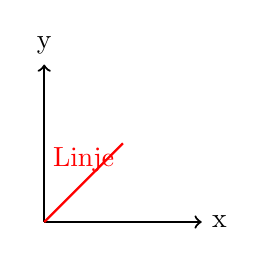
\begin{tikzpicture}
			\draw[->,thick] (0,0) -- (2,0) node[right]{x};
			\draw[->,thick] (0,0) -- (0,2) node[above]{y};
			\draw[red,thick] (0,0) -- (1,1) node[midway,above]{Linje};
		\end{tikzpicture}
	\end{frame}
	
\end{document}
